 \documentclass[11pt,a4paper]{article}
\usepackage[utf8]{inputenc}
\usepackage[slovene]{babel}
\usepackage{physics}
\usepackage{amsmath}
\usepackage{bm}
\usepackage{amsfonts}
\usepackage{amssymb}
\usepackage[left=3cm,right=3cm,top=3cm,bottom=3.8cm]{geometry}
\usepackage{caption}
\usepackage{graphicx}
\usepackage{float}
\setlength\parindent{0pt}


\title{02-Airbounce: Ideje in rešitve}
\date{}

\begin{document}

\maketitle

\section{Stabilen (vrteči) disk}
Disk zaradi vrtenja ohranja smer. Smer upora pravokotna na disk. Disk vzporeden z u.
\begin{figure}[H]
\centering
	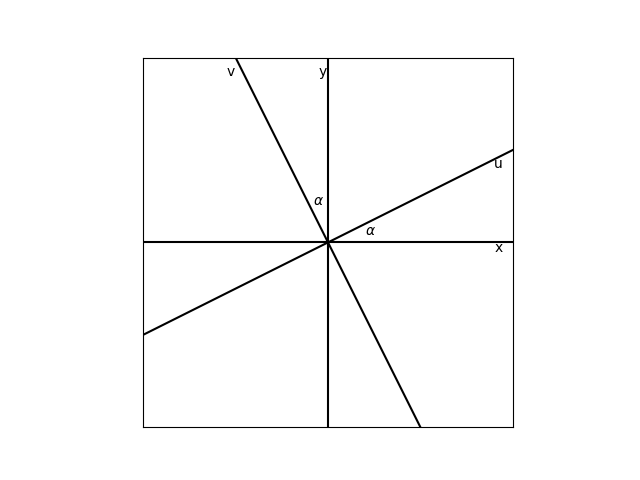
\includegraphics[width=6cm]{stabilen_disk_kot_frizbija.png}
\end{figure}

\begin{gather}
m \bm{a} = \bm{{F_g}} + \bm{F_C}\\
m \bm{a} = -mg \vu{e}_y + C v_v^2 \vu{e}_v\\
\vu{e}_v = \mqty(-\sin \alpha \\ \cos \alpha)\\
v_v = \bm{v} \cdot \vu{e}_v\\
m \mqty(v_x' \\ v_y') = -mg \mqty(0 \\ 1) + C (-v_x \sin \alpha + v_y \cos \alpha)^2 \mqty(-\sin \alpha \\ \cos \alpha)
\end{gather}
Lahko zapišem od začetka v k. sistemu u, v. Ali pa pomnožim z:
\begin{gather}
R = \mqty(\cos \alpha & \sin \alpha \\ -\sin \alpha & \cos \alpha)\\
m \mqty(v_u' \\ v_v')_{uv} = -mg \mqty(\sin \alpha \\ \cos \alpha)_{uv} + C v_v^2 \mqty(0 \\ 1)_{uv}
\end{gather}

Nadaljevanje, dve diferencialni enačbi. Rešitev s separacijo spremenljivk, (v brez dimenzijsko obliko)...

\end{document}
